\chapter{Strojeni regulator�w klasycznych}

Stworzone regulatory zosta�y wst�pnie dostrojone, po czym przeprowadzono z~ich udzia�em szereg symulacji w~tych samym warunkach testowych. Zar�wno w~przypadku regulatora PID jak i~DMC parametry zosta�y dobrane metod� in�yniersk�. Jak wiadomo, ka�dy student Automatyki i~Robotyki posiada na trzecim roku studi�w taki baga� do�wiadcze� zwi�zanych z~obydwoma algorytmami, �e optymalne parametry dla przypadk�w $1*1$ wyczuwa pod�wiadomie. Znalezione parametry regulatora PID zestawiono w~tabeli \ref{PID_params}.

\vskip 0.5cm
\begin{center}
    \begin{figure}[H]
        \makebox[\textwidth]{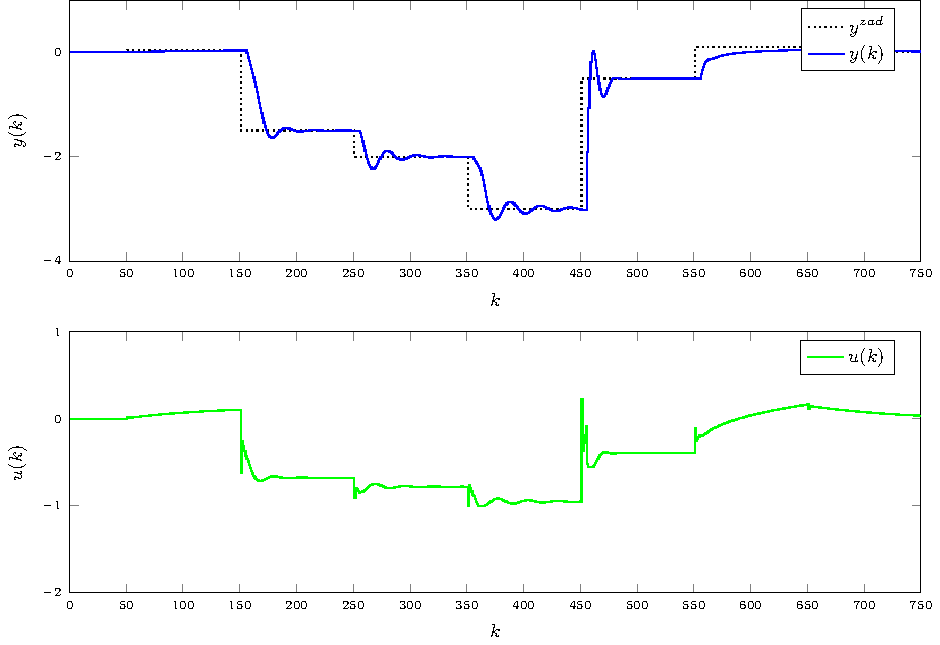
\includegraphics[width=\paperwidth]{data/exercise_6/Desired_plot_PID_number_of_fuzzy_reg_1.pdf}}
        \label{PID_experiment}
        \caption{Przebieg eksprymentu dla dobranych parametr�w regulatora PID}
    \end{figure}
\end{center}
\vskip 0.5cm

Przebiegi scenariusza testowego zosta�y przedstawione na \ref{PID_experiment}. Jak wida� jako�� regulacji jest niedoskona�a, ale bior�c pod uwag�, �e algorytm PID nie jest przeznaczony dla proces�w nieliniowych, wyniki i~tak wypadaj� stosunkowo dobrze. Sumaryczny b��d regulatora rozumiany jako suma kwadrat�w uchybu ze wszystkich chwil dyskretnych symulacji wyni�s� $\num{88.835}$. Przebieg sterowania wydaje si� dopuszczalny.


\vskip 0.5cm
\begin{center}
    \begin{figure}[H]
        \makebox[\textwidth]{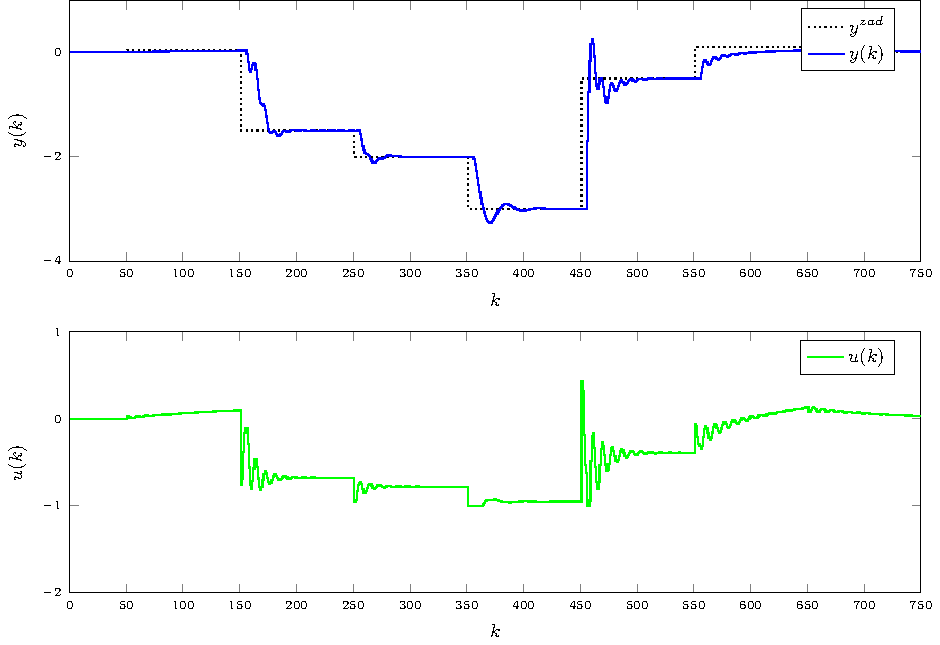
\includegraphics[width=\paperwidth]{data/exercise_6/Desired_plot_DMC_number_of_fuzzy_reg_1.pdf}}
        \label{Desired_plot_DMC_number_of_fuzzy_reg_1}
        \caption{Przebieg eksprymentu dla dobranych parametr�w regulatora DMC}
    \end{figure}
\end{center}
\vskip 0.5cm

Parametry regulatora DMC znalaz�y si� z kolei w tabeli \ref{DMC_params}. W~jego przypadku przebiegi s� �agodniejsze w~cz�ci liniowej i~troch� bardziej poszarpane po przej�ciu do obszaru liniowego. Zmiana ta zosta�a okupiona wzmo�onymi oscylacjami sterowania po wykonywanych skokach. Sumaryczny b��d regulatora wyni�s� $\num{85.7141}$, czyli nieznacznie lepiej ni� w~przypadku regulatora PID.

\vskip 0.5cm
\begin{table}[H]
    \centering
    \begin{tabular}{ | m{5em} | m{5em} |m{5em} |m{5em} | }
        \hline
        $K$ & $T_i$ & $T_d$ & $T_s$ \\
        \hline
        $\num{0.174}$ & $\num{2.3}$ & $\num{0.8}$ & $\num{0.5}$ \\
        \hline
    \end{tabular}
    \label{PID_params}
    \caption{Parametry regulator PID}
\end{table}
\vskip 0.5cm

\vskip 0.5cm
\begin{table}[H]
    \centering
    \begin{tabular}{ | m{5em} | m{5em} |m{5em} |m{5em} | }
        \hline
        $D$ & $N$ & $N_u$ & $\lambda$ \\
        \hline
        $\num{51}$ & $\num{15}$ & $\num{7}$ & $\num{0.2}$ \\
        \hline
    \end{tabular}
    \label{DMC_params}
    \caption{Parametry regulator DMC}
\end{table}
\vskip 0.5cm